\section{Actividad No 03 – Documento importantes} 
		
\begin{enumerate}
\item \textbf{Introducción}
\newline
Este es un pequeño trabajo de investigacion para el curso de Base de Datos II.
Basicamente el trabajo consta de tres partes: Los objetivos, el Marco Teorico y las Conclusiones. 

\item \textbf{Marco Teórico}
\newline
\textbf{El SCV}
\newline
Un sistema de control de versiones es una herramienta que registra todos los cambios hechos en uno o más proyectos, guardando así versiones del producto en todas sus fases del desarrollo. Las versiones son como fotografías que registran su estado en ese momento del tiempo y se van guardando a medida que se hacen modificaciones al código fuente.
\\Un sistema de control de versiones debe proporcionar:
\begin{itemize}
	\item[$*$] Mecanismo de almacenamiento de los elementos que deba gestionar.
	\item[$*$] Posibilidad de realizar cambios sobre los elementos almacenados (ej. modificaciones parciales, añadir, borrar, renombrar o mover elementos).
	\item[$*$] Registro histórico de las acciones realizadas con cada elemento o conjunto de elementos (normalmente pudiendo volver o extraer un estado anterior del producto).\end{itemize}

\begin{figure}
\begin{center}
  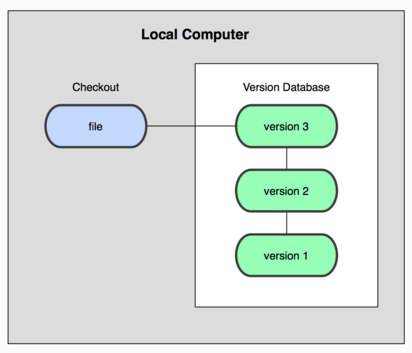
\includegraphics[width=0.9\textwidth]{Imagenes/grafico1.png}
\caption{Sistemas de Control de Versiones Locales}
\end{center}
\end{figure}

\begin{figure}
\begin{center}
  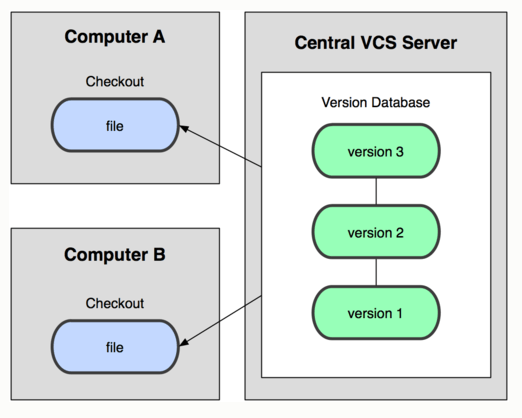
\includegraphics[width=0.9\textwidth]{Imagenes/grafico2.png}
\caption{Sistemas de Control de Versiones Centralizados}
\end{center}
\end{figure}

\begin{figure}
\begin{center}
  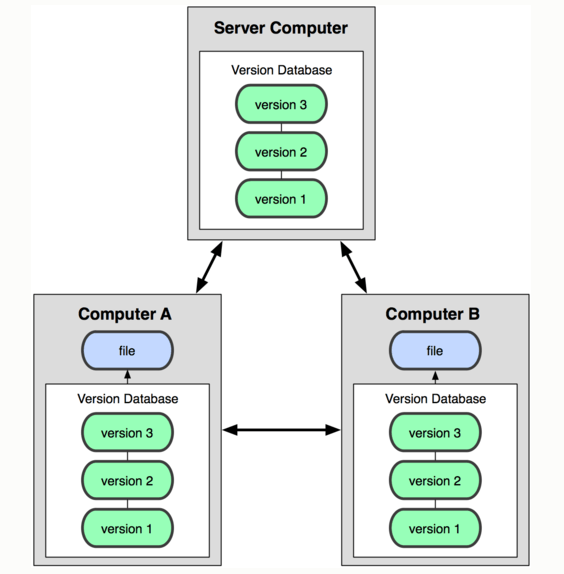
\includegraphics[width=0.9\textwidth]{Imagenes/grafico3.png}
\caption{Sistemas de Control de Versiones Distribuidos}
\end{center}
\end{figure}


\end{enumerate}



